\documentclass[11pt,a4paper]{article}

\usepackage[utf8]{inputenc}
\usepackage[T1]{fontenc}
\usepackage[margin=2.4cm]{geometry}
\usepackage{amsmath,amssymb}
\usepackage{graphicx}
\usepackage{booktabs}
\usepackage{array}
\usepackage{xcolor}
\usepackage{caption}
\usepackage{subcaption}
\usepackage{float}
\usepackage{enumitem}
\usepackage{listings}
\usepackage{siunitx}
\usepackage[hidelinks]{hyperref}

\graphicspath{{figurs/}{figures/}}

\definecolor{codebg}{gray}{0.96}
\lstset{
  basicstyle=\ttfamily\footnotesize,
  backgroundcolor=\color{codebg},
  breaklines=true,
  breakatwhitespace=false,
  columns=fullflexible,
  frame=single,
  framesep=4pt,
  xleftmargin=4pt,
  showstringspaces=false,
  literate={\%}{{\char37}}1
}

\sisetup{round-mode=places,round-precision=3,detect-weight=true}

\title{\vspace{-1.2cm}\textbf{Reproduction and Critical Study of\\ ``HTTP2vec: Embedding of HTTP Requests for\\ Detection of Anomalous Traffic''}}
\author{Data Science in Cyber --- Final Project\\
Course lecturer: Dr.\ Uri Itai}
\date{\today}

\begin{document}
\maketitle
\vspace{-0.6cm}

\begin{abstract}
\noindent
This project reproduces and critically evaluates the paper \emph{HTTP2vec: Embedding
of HTTP Requests for Detection of Anomalous Traffic} (Gniewkowski et al., 2021,
arXiv:2108.01763). The method treats a raw HTTP request as text, learns a RoBERTa
masked--language model on \emph{normal} traffic only, embeds each request as the mean
of its last hidden layers, and classifies the resulting vectors. We re--implement the
full pipeline from scratch, run it on the CSIC~2010 dataset (a seeded 40\% subset,
5~epochs), and compare seven classifiers plus a trainable MLP head. We reproduce the
paper's \emph{qualitative} central claim---RoBERTa embeddings make normal and
anomalous HTTP requests strongly separable for supervised classifiers (best
$\text{F1}=0.913$, MCC $=0.853$, ROC--AUC $=0.983$)---but we do \emph{not} reproduce
its most impressive headline numbers (near--zero false--positive rates, near--perfect
scores on CSE--CIC--IDS2018), and we show with our own experiments that the paper's
optimism about \emph{unsupervised} detection on the same embeddings is not supported
(Isolation Forest F1 $=0.45$, LOF F1 $=0.34$). We argue that several of the paper's
strongest results are driven by dataset artifacts and an unrealistic class base rate
rather than by the representation itself.
\end{abstract}

\tableofcontents
\bigskip

\noindent\textbf{Reproduced source.} M.~Gniewkowski, H.~Maciejewski, T.~Surmacz, W.~Walentynowicz,
\emph{HTTP2vec: Embedding of HTTP Requests for Detection of Anomalous Traffic}, arXiv:2108.01763v1
(2021).\\
\textbf{Reproduction repository.} \url{https://github.com/nirmanor1/cyberAno}\\
\textbf{Dataset.} CSIC~2010 HTTP dataset (Spanish Research National Council, CSIC), \url{https://www.tic.itefi.csic.es/dataset/}

\clearpage

\section{Summary of the Source}
\label{sec:summary}

\subsection{The problem being addressed}
HTTP is the transport used by the large majority of web traffic, and therefore by the
majority of web attacks: SQL injection, cross--site scripting (XSS), CRLF injection,
buffer overflows, information gathering, and file disclosure all travel inside HTTP
requests. The paper addresses \emph{web attack / anomaly detection}: given a raw HTTP
request, decide whether it is legitimate (\emph{normal}) or an attack (\emph{anomaly}).
This is a Web Application Firewall / Intrusion Detection System (IDS) problem.

\subsection{Why the problem is important}
According to the OWASP Top~Ten, injection is a top web threat. Classic defences are
either \emph{signature/rule--based} (e.g.\ Snort) or trained on \emph{hand--crafted
features}. Rule--based systems require constant expert maintenance and miss novel
attacks; hand--crafted features are brittle and encode analyst bias. An accurate,
low--maintenance detector that learns the structure of traffic directly would reduce
both missed attacks (breaches) and false alarms (analyst fatigue), and, if
\emph{interpretable}, would also help post--incident analysis.

\subsection{The proposed solution}
The core idea is to treat an HTTP request as a sentence in an (artificial) language and
borrow modern NLP representation learning. Concretely, the authors:
\begin{enumerate}[nosep,leftmargin=1.4em]
  \item train a \textbf{byte--level BPE (BBPE) tokenizer} on all traffic, so there is no
        out--of--vocabulary problem for adversarial payloads;
  \item train a \textbf{RoBERTa} masked--language model (MLM) \emph{only on normal
        traffic}, so it learns what ``normal'' HTTP looks like;
  \item \textbf{embed} each request as the mean over its lines of the concatenation of
        the last four hidden layers (a $4\times768=3072$--dimensional vector);
  \item \textbf{classify} the embeddings with standard scikit--learn models: Logistic
        Regression (LR), Random Forest (RF) and linear Support Vector Classification
        (SVC).
\end{enumerate}
Two further contributions are emphasised: (i) \textbf{interpretability}, via a
token--removal procedure that scores how much each token pushes a request across the
classifier's decision boundary; and (ii) \textbf{visualisation / clustering} of the
embedding space with t--SNE.

\subsection{The dataset used}
The paper evaluates three datasets: \textbf{CSIC~2010} (the canonical text--form HTTP
attack dataset), \textbf{CSE--CIC--IDS2018} (extracting web attacks from packet
captures) and \textbf{UMP} (a dataset the authors collected themselves). Each dataset is
split into a \emph{training} part (normal only, used to fit RoBERTa) and an
\emph{inference} part (normal $+$ anomalous, used for classification). For CSIC~2010 the
paper uses $36{,}000$ normal training requests, $36{,}000$ normal inference requests and
$25{,}065$ anomalous inference requests (Table~1 of the paper). \textbf{Our reproduction
focuses on CSIC~2010}, which is the only one of the three available in a ready--to--use
text form.

\subsection{The methodology employed}
The RoBERTa model is the ``base''--style configuration but shrunk to 6 layers, hidden
size 768, 12 attention heads, maximum sequence length 512, trained for 10 epochs with
batch size 32 and 15\% masked tokens. Evaluation follows a \textbf{stratified 5--fold
cross--validation}, reporting \textbf{F1}, \textbf{MCC}, and \textbf{FPR@TPR}
($\text{FPR}_{90}$ and $\text{FPR}_{99}$: the false--positive rate required to catch
90\% / 99\% of attacks). The headline CSIC~2010 result is $\text{F1}=0.969$ (SVC) with
$\text{FPR}_{99}=4.2\%$, and a ``perfect'' classifier ($\text{F1}=0.999$) on
CSE--CIC--IDS2018.

\section{Critical Evaluation of the Author's Claims}
\label{sec:critical}

This section is the heart of the project. We enumerate the paper's main claims and test
each against the evidence in the paper and against our own reproduction
(Sections~\ref{sec:results}--\ref{sec:error}). A compact verdict table is given at the
end (Table~\ref{tab:claims}).

\subsection{Claim 1 --- RoBERTa embeddings give state--of--the--art supervised detection}
\textbf{Supported qualitatively; the exact numbers are optimistic.} Our reproduction
confirms the \emph{direction} of this claim strongly: even on a 40\% subset trained for
only 5~epochs, simple classifiers on the embeddings reach $\text{F1}=0.91$,
$\text{MCC}=0.85$ and $\text{ROC--AUC}=0.98$ (Table~\ref{tab:holdout}). The linear SVC
working well tells us the classes are close to \emph{linearly separable} in the
3072--dimensional space---exactly the paper's argument. However, the paper's specific
CSIC~2010 numbers are noticeably better than ours: SVC $\text{F1}=0.969$ vs our
$0.910$, and, more importantly, $\text{FPR}_{99}=4.2\%$ vs our $\approx21.5\%$. The
gap on the low--false--positive metrics---the ones that matter operationally---is large
(Section~\ref{sec:paper-vs-repro}). Calling this ``state--of--the--art'' is also
weakened by the leakage issues discussed under Claim~4.

\subsection{Claim 2 --- The representation is learned ``unsupervised'' and suits real,
label--free deployments}
\textbf{Misleading as stated.} The \emph{representation} (RoBERTa) is indeed learned
without labels---on normal traffic only---but the \emph{detection} in the paper is fully
\emph{supervised}: LR/RF/SVC are trained on labelled normal $+$ anomalous embeddings. The
paper's conclusion further speculates that \emph{unsupervised} detection ``is likely to
be effective'' on these embeddings. We tested this directly by fitting an Isolation
Forest and a Local Outlier Factor detector on normal--only embeddings and scoring the
mixed set. Both are far weaker than the supervised models: Isolation Forest reaches only
$\text{F1}=0.45$ ($\text{ROC--AUC}=0.75$) and LOF $\text{F1}=0.34$
(Table~\ref{tab:holdout}). So on our evidence the embeddings are excellent \emph{features
for a supervised classifier} but do \emph{not} yet support effective unsupervised
detection; the paper's optimistic framing is not substantiated.

\subsection{Claim 3 --- The classes are ``well separated'' and form clean clusters in 2D}
\textbf{Only partially supported.} The paper shows t--SNE plots and states that classes
are ``well separated even in a lower space''. Our t--SNE (Figure~\ref{fig:tsne}) does show
clear \emph{cluster structure}---requests group by endpoint/type---and one large,
almost purely normal cluster. But many peripheral clusters are visibly \emph{mixed}
(red and blue together). The strong separability the classifiers exploit lives in the
full 3072--dimensional space, not in the 2D projection; the visualisation somewhat
oversells the ``well separated'' narrative. t--SNE is also a non--linear, perplexity
--dependent embedding and should not be read as evidence of linear separability.

\subsection{Claim 4 --- Near--perfect results on CSE--CIC--IDS2018 demonstrate the method}
\textbf{This is essentially a data artifact, and the authors say so.} The paper reports
$\text{F1}=0.999$ on IDS2018 and, commendably, investigates \emph{why}: the interpretability
analysis reveals that the tokens \texttt{Accept} and \texttt{Accept--Encoding} are
``highly related to the anomaly subset'' because those header lines appear in nearly
unchanged form in almost every attack. That is a textbook \emph{spurious correlation /
data leakage}: the model learns an artifact of how the attack traffic was generated
(a scanner with fixed headers), not a property of attacks. The same paper notes an
analogous artifact in CSIC~2010---every anomalous request ends with \texttt{\textbackslash
n} rather than \texttt{\textbackslash r\textbackslash n}. A ``perfect'' score built on
such artifacts is not evidence of generalisation, and the paper's own conclusion (``the
dataset is really simple to classify or we made some mistakes'') implicitly concedes this.
We did not reproduce IDS2018 (it is not in ready text form), but we flag that this
headline number should not be read as method quality.

\subsection{Claim 5 --- The method is interpretable}
\textbf{Plausible and a genuine strength, but not reproduced here.} The token--removal
attribution is a reasonable, model--agnostic explanation technique and is one of the
paper's more original contributions; the examples shown (SQL keywords such as
\texttt{DROP}/\texttt{SELECT}/\texttt{FROM} dominating an SQL--injection request) are
convincing. We deliberately kept this out of scope---our reproduction targets the
\emph{classification} claims---so we neither confirm nor refute the exact attribution
scores. We note only that the technique's cost (re--embedding one document per token) is
high for long requests.

\subsection{Is the evaluation methodology appropriate?}
Mostly yes, with important caveats. \textbf{Good:} stratified $k$--fold CV; the correct
choice of threshold--aware metrics (F1, MCC, FPR@TPR) instead of bare accuracy; and,
crucially, the separation of the \emph{normal--training} set (for the LM) from the
\emph{normal--inference} set (for classification), which we verified in the code and
which avoids the most obvious form of leakage. \textbf{Caveats:} (i) the reported class
base rate ($\approx$41\% anomalies) is wildly higher than any real deployment, which
inflates precision, F1 and accuracy relative to production
(Section~\ref{sec:eda-balance}); (ii) CSIC~2010 contains heavy near--duplication and
method--level giveaways (Section~\ref{sec:eda-dupes}) that make the task easier than
real traffic; and (iii) the CAE baseline the paper compares against ``converged to a
local minimum \dots and did not learn'', so the comparison to prior work is partly
against a model the authors could not make work.

\subsection{Are the conclusions justified?}
The narrow conclusion---\emph{RoBERTa embeddings of HTTP requests are strong features for
supervised web--attack detection}---is justified and we reproduce it. The broader
conclusions---SOTA performance, effectiveness of \emph{unsupervised} detection, and
clean 2D separability---are only partially justified: they are inflated by dataset
artifacts, an unrealistic base rate, and (for the unsupervised claim) contradicted by our
experiments. The paper is unusually honest about its own artifacts, which is to its
credit, but the abstract and conclusion do not carry those caveats forward.

\section{Exploratory Data Analysis (EDA)}
\label{sec:eda}

All EDA is performed on a \emph{descriptive} feature frame of the inference set: one row
per request, $24{,}426$ rows $\times$ 16 columns of human--readable, model--agnostic
attributes (lengths, counts, ratios, entropy and two attack--signature flags) plus the
label. These descriptive features exist \emph{only} for EDA and error analysis---they are
not the features the model uses (those are the RoBERTa embeddings,
Section~\ref{sec:fe}).

\subsection{Data loading, inspection and quality}
\label{sec:eda-dupes}
The loader returns three views matching the paper: \texttt{lm\_train} (normal only,
$14{,}400$), \texttt{inference} (normal $+$ anomaly, $24{,}426$) and a tokenizer corpus
(all traffic, $38{,}826$). We verified in code that the normal inference requests come
from a \emph{different} file (\texttt{normalTrafficTest.txt}) than the LM--training
normals (\texttt{normalTrafficTraining.txt}), so there is no train/inference leakage on
the normal side. Data--quality checks returned:
\begin{itemize}[nosep,leftmargin=1.4em]
  \item \textbf{Missing values:} none in any column.
  \item \textbf{Constant / single--value columns:} none.
  \item \textbf{Exactly duplicated feature columns:} none.
  \item \textbf{Fully duplicated rows:} $15{,}678$ of $24{,}426$ ($\approx$64\%).
\end{itemize}
The last figure is striking and important. It does \emph{not} mean 64\% of the raw
requests are identical---rather, that a large majority of requests collapse to the
\emph{same descriptive fingerprint} (same method, lengths, ratios, flags). CSIC~2010 is
generated by exercising a single e--commerce application, so requests are highly
templated. Practically this means the effective diversity of the data is far lower than
$24{,}426$, cross--validation folds share near--identical patterns, and reported
performance is optimistic relative to heterogeneous real traffic. The columns and the
default positional index are sensible: CSIC has no natural key (no request id, no
timestamp), so a positional index that aligns row~$i$ with request~$i$ is the right
choice and is what we use for error analysis (Section~\ref{sec:error}).

\subsection{Class balance (prevalence) and its real--world meaning}
\label{sec:eda-balance}
The inference set is $14{,}400$ normal ($59\%$) and $10{,}026$ anomaly ($41\%$). This is
only mildly imbalanced, so \emph{accuracy} is not catastrophically misleading here---but
it is deeply \textbf{unrealistic}. In production, web attacks are a tiny fraction of
traffic (often $\ll1\%$). At a realistic base rate, a detector with our reproduced
$\text{FPR}_{99}\approx21.5\%$ would drown analysts in false positives: to catch 99\% of
attacks it would misflag more than a fifth of \emph{all} benign traffic, and because
benign traffic dominates, precision would collapse far below the $0.92$ we measure at
41\% prevalence. The authors do not correct for this base--rate mismatch. Consequently we
de--emphasise accuracy and prefer MCC, ROC--AUC and FPR@TPR, which are either
imbalance--robust or explicitly operational (Section~\ref{sec:metrics}).

\subsection{Feature distributions by class}
Figure~\ref{fig:dist} shows six representative features split by class.
\texttt{target\_length}, \texttt{body\_length} and \texttt{pct\_encoding\_ratio} are
strongly right--skewed: most requests are short with little percent--encoding, but a
heavy anomaly tail extends to long, heavily encoded payloads. \texttt{shannon\_entropy}
is the cleanest single--feature separator---anomalies shift towards higher character
entropy---and \texttt{n\_query\_params} shows a discrete anomaly spike at high parameter
counts. These are exactly the shapes one expects from injection/obfuscation payloads.

\begin{figure}[H]
  \centering
  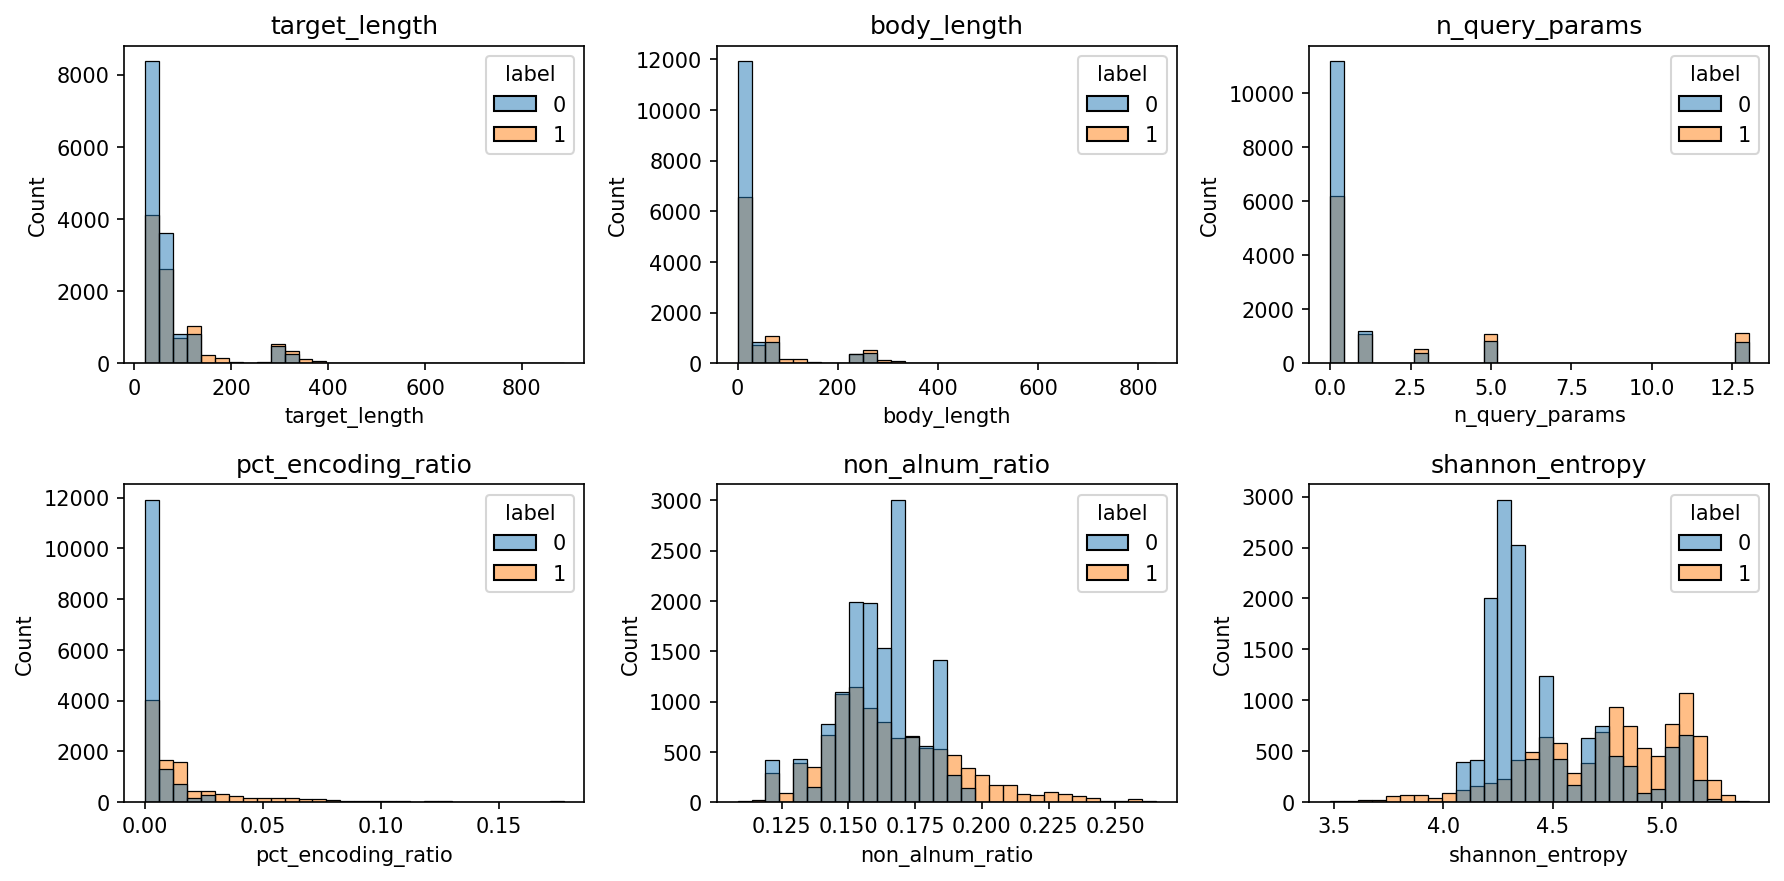
\includegraphics[width=\linewidth]{2_2_feature_distributions.png}
  \caption{Distributions of six descriptive features by class ($0=$ normal, $1=$
  anomaly). Lengths and percent--encoding are heavy--tailed; entropy and query--parameter
  count show the clearest class shift.}
  \label{fig:dist}
\end{figure}

\subsection{Correlation analysis and choice of coefficient}
\label{sec:eda-corr}
We report \textbf{Spearman} rank correlation (Figure~\ref{fig:corr}) as the primary
measure. The three candidates studied in the course capture different relationships:
\begin{itemize}[nosep,leftmargin=1.4em]
  \item \textbf{Pearson} measures \emph{linear} association between continuous variables;
        it assumes roughly linear, normal--ish data and is sensitive to outliers.
  \item \textbf{Spearman} is the Pearson correlation of the \emph{ranks}; it captures any
        \emph{monotonic} relationship and is robust to outliers and non--normality.
  \item \textbf{Kendall} ($\tau$) is also rank--based, counting concordant vs discordant
        pairs; it is preferred for small samples or many ties and is more conservative.
\end{itemize}
Our descriptive features are heavily skewed, non--normal and full of legitimate outliers
(long attack payloads), and we care about \emph{monotonic} ``more of this $\Rightarrow$
more likely an attack'' relationships rather than strict linearity. Spearman is therefore
the appropriate choice; Pearson would be distorted by the heavy tails and Kendall is
unnecessary given the large $n$.

\begin{figure}[H]
  \centering
  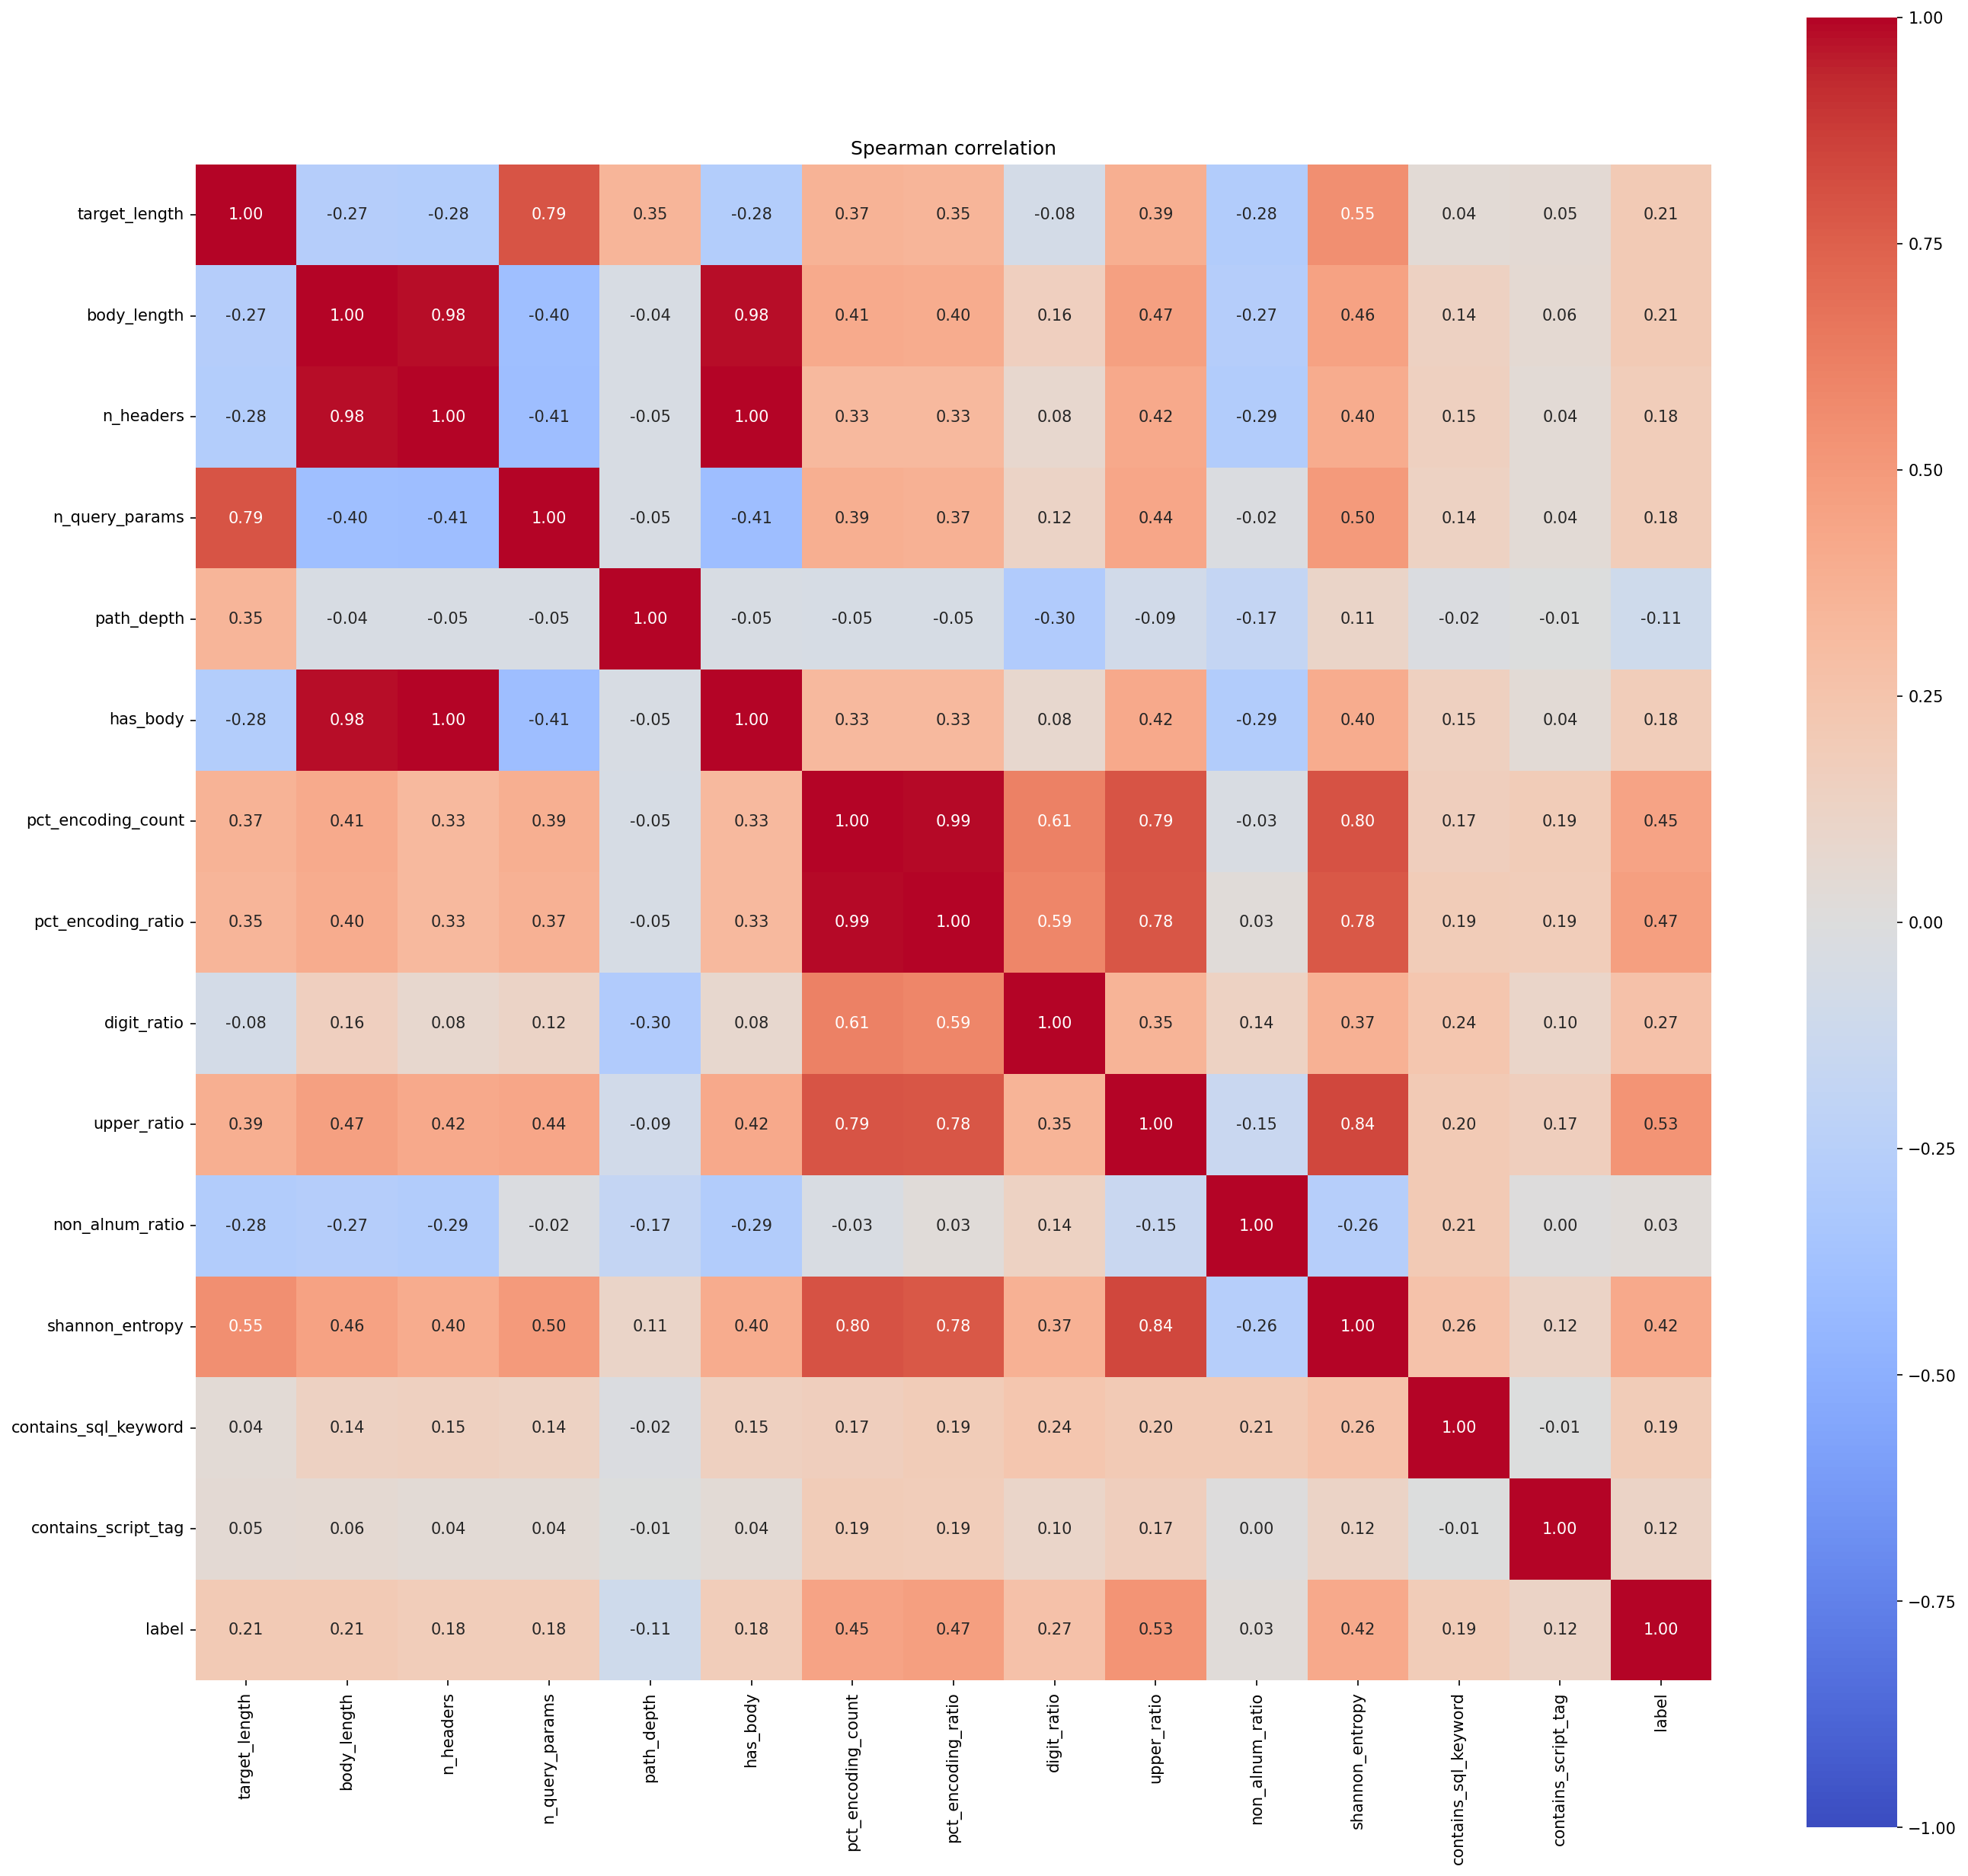
\includegraphics[width=0.92\linewidth]{2_3_correlation_spearman.png}
  \caption{Spearman correlation heatmap of the descriptive features and the label.
  Note the near--perfectly collinear block \{\texttt{body\_length}, \texttt{n\_headers},
  \texttt{has\_body}\} and the pair \{\texttt{pct\_encoding\_count},
  \texttt{pct\_encoding\_ratio}\}.}
  \label{fig:corr}
\end{figure}

\noindent\textbf{Association with the label.} The descriptive features most correlated
with ``anomaly'' are \texttt{upper\_ratio} ($\rho=0.53$), \texttt{pct\_encoding\_ratio}
($\rho=0.47$), \texttt{shannon\_entropy} ($\rho=0.42$) and \texttt{digit\_ratio}
($\rho=0.27$). These are \emph{practically}, not merely statistically, significant: a
$\rho$ of $0.5$ on a single cheap feature is a meaningful monotonic signal. The
cybersecurity reading is direct---SQL keywords (\texttt{DROP}, \texttt{SELECT},
\texttt{UNION}) and XSS tags inject uppercase letters and unusual symbols, evasion relies
on percent--encoding, and both raise character entropy. Even the crudest features carry
attack signal, which is \emph{why} a contextual embedding that subsumes them works so
well.

\subsection{Redundancy spotted during EDA}
The heatmap immediately exposes redundancy (revisited in Section~\ref{sec:fe-redundancy}):
\texttt{body\_length}, \texttt{n\_headers} and \texttt{has\_body} are almost perfectly
collinear ($\rho=0.98$--$1.00$), because in CSIC a request has a body iff it is a POST,
which also carries the extra headers; \texttt{pct\_encoding\_count} and
\texttt{pct\_encoding\_ratio} are $\rho=0.99$; and \texttt{upper\_ratio} tracks
\texttt{shannon\_entropy} at $\rho=0.84$.

\subsection{Group--by / crosstab: an accidental label proxy}
Cross--tabulating the HTTP method against the label reveals a dataset artifact:

\begin{table}[H]
  \centering
  \begin{tabular}{lrrr}
    \toprule
    Method & Normal & Anomaly & Anomaly share\\
    \midrule
    GET  & $11{,}119$ & $6{,}040$ & $35\%$\\
    POST & $3{,}281$  & $3{,}818$ & $54\%$\\
    PUT  & $0$        & $168$     & $100\%$\\
    \bottomrule
  \end{tabular}
  \caption{HTTP method vs label on the inference set. \texttt{PUT} appears
  \emph{only} in anomalies---a partial label giveaway present in the raw data.}
  \label{tab:crosstab}
\end{table}

\noindent \texttt{PUT} occurs in $168$ requests, \emph{all} of them anomalous. A model can
therefore ``cheat'' on those requests using the verb alone. This is another reason the
task is easier on CSIC than in the wild and reinforces the artifact theme from Claim~4.

\subsection{Outliers and the (absent) temporal dimension}
\texttt{target\_length} has median $50$ but a 99th percentile of $340$ and a maximum of
$886$; \texttt{body\_length} is similar. These extreme values are overwhelmingly attack
payloads, so here \emph{outliers are signal, not noise}---we keep them rather than
winsorising. Finally, CSIC~2010 has \textbf{no timestamps}, so a temporal / concept--drift
analysis is impossible. This is a real limitation: production IDS must cope with drift
(new endpoints, changing user behaviour), and neither the dataset nor the paper can speak
to it. This aligns with world knowledge that attack and traffic mixes change over time.

\section{Feature Engineering Analysis}
\label{sec:fe}

\subsection{Was feature engineering performed, and on which features?}
Yes---but the paper's thesis is precisely that the feature engineering should be
\emph{learned}, not hand--crafted. There are two distinct feature sets in this project:
\begin{enumerate}[nosep,leftmargin=1.4em]
  \item \textbf{The model features (the paper's contribution):} the 3072--dimensional
        RoBERTa embedding of each request. This is the only input the classifiers see.
  \item \textbf{The descriptive features (our EDA add--on):} the 15 human--readable
        attributes of Section~\ref{sec:eda}. They are never fed to the model; they exist
        to make the data inspectable and the errors explainable.
\end{enumerate}

\subsection{Transformations applied, why, and their effect}
\paragraph{Encoding (text $\rightarrow$ numeric): byte--level BPE.} Raw requests are
strings, so an encoding step is unavoidable. The paper uses a \emph{byte--level} BPE
tokenizer trained on all traffic. \emph{Why:} operating on bytes eliminates the
out--of--vocabulary problem---percent--encoded bytes, random tokens in payloads and
rare characters all decompose into known sub--tokens---while keeping the vocabulary small
($30{,}000$). Training the tokenizer on \emph{all} traffic (not just normal) is a
deliberate choice so that short/rare tokens are not themselves treated as anomalous.
\emph{Effect:} a robust, lossless encoding of adversarial text, which is the precondition
for everything downstream.

\paragraph{Feature creation: contextual embeddings.} Each request line is passed through
RoBERTa; the last four hidden layers are concatenated ($4\times768$), mean--pooled over
tokens, and the per--line vectors are averaged into one request vector. \emph{Why the
last four layers:} different transformer layers encode different levels of abstraction, and
concatenating the top layers is a well--known feature--based BERT recipe that empirically
beats using the final layer alone. \emph{Why mean pooling / line averaging:} it yields a
fixed--length vector regardless of request length and is order-- and length--robust.
\emph{Effect:} the resulting space is close to linearly separable (the linear SVC scores
$\text{F1}=0.91$), which is the central empirical payoff.

\paragraph{Scaling: standardisation.} Embedding dimensions are standardised
(\texttt{StandardScaler}, zero mean/unit variance) inside the linear models, the anomaly
detectors and the MLP head; the tree ensembles (Random Forest, gradient boosting) skip
scaling because they are scale--invariant. \emph{Why:} logistic regression, linear SVC,
KNN and the distance/density--based detectors are all sensitive to feature scale;
unscaled dimensions with large variance would dominate. \emph{Effect:} required for the
linear and distance--based models to behave; a pure convenience for trees, hence omitted
there.

\paragraph{Dimensionality reduction: used for analysis, not for classification.} The
paper keeps the full 3072--dimensional vector for classification and explicitly lists its
size as a limitation (``dimensionality \dots ca.\ 3000 \dots affects training and
inference time''). We make this concrete with PCA (Figure~\ref{fig:pca}): the first
principal component already explains $\approx60\%$ of the variance, and only
\textbf{$\approx$13--14 components} are needed to reach 90\%. In other words the intrinsic
dimensionality is an order of magnitude smaller than 3072---the representation is
\emph{highly redundant}. t--SNE (Figure~\ref{fig:tsne}) is used only for 2D visualisation,
never as a classifier input.

\begin{figure}[H]
  \centering
  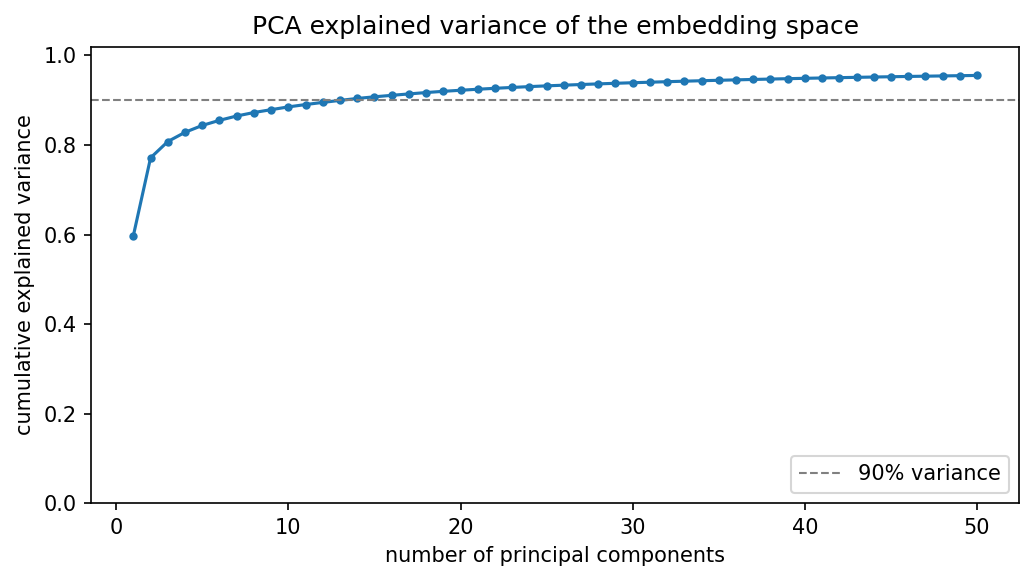
\includegraphics[width=0.78\linewidth]{3_3_pca_explained_variance.png}
  \caption{Cumulative PCA explained variance of the 3072--dimensional embedding space.
  About 13--14 components already capture 90\% of the variance, quantifying the paper's
  ``too large a representation'' limitation.}
  \label{fig:pca}
\end{figure}

\subsection{Is there redundancy, how would you spot it, and how would you tackle it?}
\label{sec:fe-redundancy}
Redundancy is present at both feature levels, and we used four complementary tools to spot
it:
\begin{enumerate}[nosep,leftmargin=1.4em]
  \item \textbf{Constant--column check} (variance $=0$): none here, but the cheapest first
        screen.
  \item \textbf{Exact duplicate--column check} (compare columns as vectors): none exactly
        identical.
  \item \textbf{Correlation heatmap} (Section~\ref{sec:eda-corr}): exposes the collinear
        blocks \{\texttt{body\_length}, \texttt{n\_headers}, \texttt{has\_body}\}
        ($\rho\!\approx\!1$) and \{\texttt{pct\_encoding\_count},
        \texttt{pct\_encoding\_ratio}\} ($\rho=0.99$).
  \item \textbf{PCA} (Figure~\ref{fig:pca}): quantifies redundancy in the
        \emph{embedding} space, where per--dimension correlation is not human--readable.
\end{enumerate}
\textbf{How to tackle it.} For the descriptive features: drop all but one member of each
collinear group, or replace the group with a single principal component. For the embedding:
apply PCA / feature agglomeration to compress $3072\!\rightarrow\!\sim\!50$ dimensions with
negligible loss (directly addressing the paper's stated cost limitation), and/or rely on
$L_1$/$L_2$ regularisation, which the linear models already provide, to damp redundant
directions. Tree ensembles are inherently tolerant of correlated inputs. Reducing the
dimensionality would also speed up the KNN, Isolation Forest and LOF detectors, whose
distance computations degrade in high dimensions (the ``curse of dimensionality'').

\subsection{Was the feature engineering meaningful? Mathematical and security intuition}
\textbf{Mathematically:} self--attention lets RoBERTa encode each token \emph{in
context}, so the same symbol (the paper's example is ``\texttt{/}'') maps to different
vectors depending on its neighbours. Averaging contextual token vectors yields a smooth
request representation in which semantically similar requests are near one another under
Euclidean distance; a hyperplane can then separate ``normal--shaped'' from
``attack--shaped'' regions, which is why a \emph{linear} classifier suffices.
\textbf{From a security standpoint:} the descriptive analysis showed that attacks differ
from normal traffic in uppercase ratio, percent--encoding and entropy---all local,
token--level phenomena that a contextual language model captures far more richly than any
fixed feature. The embedding effectively learns a data--driven superset of the
hand--crafted signatures an analyst would otherwise maintain by hand. So yes, the feature
engineering is meaningful: it converts an intractable string--matching problem into a
well--behaved geometry problem.

\subsection{Additional features that could improve performance}
\begin{itemize}[nosep,leftmargin=1.4em]
  \item \textbf{Response--side signals} (status code, response size, latency) from server
        access/error logs---the paper itself flags this as future work; a $500$/$302$
        pattern is a strong post--hoc attack signal.
  \item \textbf{Structural / template features:} URL path template (endpoint identity),
        parameter--name sets, and header order/casing, which capture ``this request does
        not fit any known endpoint schema''.
  \item \textbf{Cheap text baselines fused with the embedding:} character $n$--gram
        TF--IDF, which prior work (and CSIC baselines) show is already competitive and is
        essentially free.
  \item \textbf{Rate / session features} (requests per client per second) to catch
        brute--forcing and scanning, which are invisible at the single--request level.
  \item \textbf{A domain--pretrained language model:} pretraining on large corpora of
        HTTP/URLs before fine--tuning on CSIC would likely improve the embedding,
        especially in the low--data regime we used.
\end{itemize}
A word of caution consistent with Claim~4: features such as the raw \texttt{\textbackslash
r\textbackslash n} terminator or fixed \texttt{Accept} headers \emph{would} boost CSIC /
IDS2018 scores but only by exploiting generation artifacts; they should be avoided, not
added.

\section{Reproducibility Analysis}
\label{sec:repro}

\subsection{Can the code be executed?}
Yes. Because we could not locate an official public code release from the authors, we
\emph{re--implemented} the full HTTP2vec pipeline as a small, modular Python package
(\texttt{src/http2vec}) and drove it from a Jupyter notebook. The notebook ran
end--to--end on a Google Colab GPU (CUDA): it clones the repository, installs the package,
downloads CSIC~2010, trains the tokenizer and RoBERTa MLM, computes embeddings, trains all
classifiers, and writes every figure and metric table. All results in this report come
from that single executed run.

\subsection{Are all required files and dependencies available?}
Dependencies are declared in \texttt{pyproject.toml} / \texttt{requirements.txt}
(\texttt{torch}, \texttt{transformers}, \texttt{tokenizers}, \texttt{scikit--learn},
\texttt{numpy}, \texttt{pandas}, \texttt{matplotlib}, \texttt{seaborn}). The version
constraints are conservative \emph{floors} rather than exact pins, so a future
incompatible release could in principle break the run; pinning the exact
\texttt{pip freeze} would make it byte--for--byte reproducible. The CSIC~2010 raw files are
deliberately \emph{not} committed (they contain real attack payloads); the repository
provides a download helper and clear instructions, and the loader raises an explicit error
listing the missing files if they are absent. Determinism is supported: a fixed seed
($42$) is threaded through data subsetting, the train/test splits, the MLM trainer and the
MLP head.

\subsection{Are there hidden preprocessing steps?}
Nothing is hidden---the whole pipeline is explicit in the configuration object---but two
preprocessing choices are subtle and materially affect results:
\begin{enumerate}[nosep,leftmargin=1.4em]
  \item \textbf{CR/LF handling.} Our parser treats CR and LF strictly as line separators
        and strips a trailing \texttt{\textbackslash r} from every line. This has an
        important side effect: it \emph{removes} the ``anomalies end in
        \texttt{\textbackslash n}, not \texttt{\textbackslash r\textbackslash n}''
        artifact that the paper identified as making CSIC easy. Our reproduction is thus a
        \emph{cleaner, harder} test than the original, which is one plausible reason our
        numbers are lower (Section~\ref{sec:paper-vs-repro}).
  \item \textbf{Subset and epochs (a hardware--imposed limitation).} The executed run used
        a seeded \textbf{40\% subset} of each file and \textbf{5 epochs} (vs the paper's
        full data and 10 epochs). This was \emph{not} a modelling preference but the
        practical ceiling of our environment: the whole pipeline was run in a single
        \textbf{Google Colab} session on a \textbf{T4 GPU (16\,GB)}, where it took almost
        \textbf{4 hours} end--to--end and peaked at \textbf{15.5 of the 16\,GB} of GPU
        memory. Larger fractions or more epochs would have exceeded either the session
        time limit or the T4's memory, so 40\%/5~epochs were the largest settings that
        completed reliably. This is a documented, intentional scaling--down---not a hidden
        step---but it is a genuine limitation of \emph{our} reproduction (distinct from the
        paper's own limitations) and must be kept in mind when comparing to the paper,
        whose full run used two RTX~2080Ti GPUs for about 7~hours.
\end{enumerate}

\subsection{Overall reproducibility}
\textbf{The paper is reproducible in spirit but not to the digit.} We reproduced its
central qualitative claim with an independent implementation, which is the strong form of
reproducibility. Exact numeric reproduction is hindered by: the absence of official code;
sensitivity to language--model training details (epochs, data size, library versions,
mixed precision); the high variance of tail metrics such as $\text{FPR}_{99}$; and the
artifact--handling differences above. The paper also reports a heavy cost (about 7~hours on
two RTX~2080Ti GPUs for CSIC~2010), which is itself a reproducibility barrier, and it
candidly documents a failed reproduction of the CAE baseline it compares against---a useful
honesty signal, but also a reminder that ``irreproducible without the original source
code'' is a real risk in this literature.

\section{Experimental Results}
\label{sec:results}

\subsection{Experimental setup and the modifications we introduced}
Our reproduction reuses the paper's architecture and protocol but adds several
experiments to stress--test the claims. The run reported here used a seeded 40\% subset of
CSIC~2010, a RoBERTa MLM (6 layers, hidden $768$, 12 heads, intermediate $3072$, vocab
$30{,}000$, max length $512$) trained for 5 epochs (batch $32$, learning rate
$5\times10^{-5}$, $15\%$ masking, weight decay $0.01$, warmup $0.06$, mixed precision on
GPU), and $3072$--dimensional embeddings (concatenation of the last four hidden layers,
mean--pooled). \textbf{Compute environment.} Everything ran in one Google Colab session on
a single \textbf{T4 GPU (16\,GB)}, taking almost \textbf{4 hours} end--to--end and using
up to \textbf{15.5\,GB} of the 16\,GB of GPU memory; the 40\%/5--epoch budget was dictated
by this ceiling rather than chosen for modelling reasons (see the limitation noted in
Section~\ref{sec:repro}). Beyond the paper we:
\begin{itemize}[nosep,leftmargin=1.4em]
  \item added two more supervised classifiers---\textbf{gradient boosting} and
        \textbf{KNN}---to the paper's LR/RF/SVC, to see whether performance is specific to
        the paper's three models;
  \item added a second unsupervised detector, \textbf{Local Outlier Factor}, alongside an
        \textbf{Isolation Forest}, to test the paper's unsupervised speculation;
  \item added a small trainable \textbf{MLP head} over the frozen embeddings (a
        ``fine--tune--like'' extension);
  \item introduced a single \textbf{shared, seeded, stratified holdout} (70/30) so that
        every model---supervised, unsupervised and the MLP---is scored on \emph{exactly
        the same} test set for a fair head--to--head comparison (the paper reports CV for
        its three models only);
  \item added a \textbf{PCA} analysis of the embedding space (Section~\ref{sec:fe}).
\end{itemize}
We report both the paper's protocol (stratified 5--fold CV) and the shared holdout.

\subsection{The RoBERTa language model}
Figure~\ref{fig:train} shows the MLM learning curve. The training loss falls sharply from
$\approx10.3$ to $\approx1.0$ and then plateaus; the per--epoch validation loss (on a
seeded 5\% held--out slice of \emph{normal} traffic) tracks it down to $\approx0.9$ and
never turns back up. This indicates the model learned the structure of normal HTTP without
obvious overfitting, even in the reduced 5--epoch budget. The corresponding perplexity
($e^{\text{loss}}$) drops by orders of magnitude, confirming the language model is
genuinely predictive of masked tokens in normal traffic.

\begin{figure}[H]
  \centering
  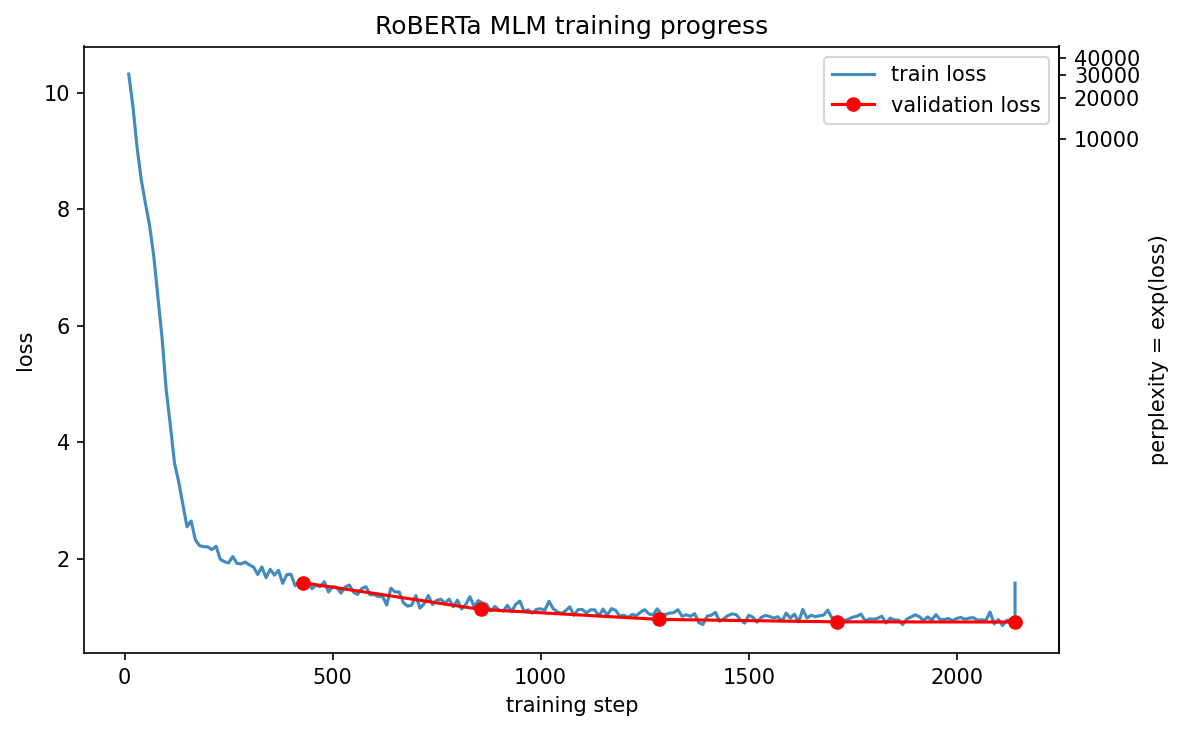
\includegraphics[width=0.82\linewidth]{3_1_training_curve.png}
  \caption{RoBERTa MLM training progress: per--step training loss (blue) and per--epoch
  validation loss (red), with a perplexity axis on the right. Steady convergence with the
  validation loss tracking training loss indicates learning without overfitting.}
  \label{fig:train}
\end{figure}

\subsection{Evaluation metrics: definitions and why they matter here}
\label{sec:metrics}
We choose metrics deliberately for an imbalanced, cost--asymmetric security task rather
than reporting a fixed list. Let TP, FP, TN, FN be the confusion--matrix counts with the
\emph{anomaly} as the positive class.

\begin{itemize}[nosep,leftmargin=1.4em]
  \item \textbf{Precision} $=\dfrac{\text{TP}}{\text{TP}+\text{FP}}$: of the requests we
        flag as attacks, how many really are. Low precision $\Rightarrow$ many false
        alarms $\Rightarrow$ analyst fatigue and eventual alert--muting.
  \item \textbf{Recall (TPR)} $=\dfrac{\text{TP}}{\text{TP}+\text{FN}}$: of the real
        attacks, how many we catch. Low recall $\Rightarrow$ missed attacks $\Rightarrow$
        breaches. This is usually the costlier error in an IDS.
  \item \textbf{F1} $=\dfrac{2\,\text{PR}}{\text{P}+\text{R}}$: harmonic mean of precision
        and recall; a single number that punishes ignoring either.
  \item \textbf{$\text{F}_\beta$}
        $=\dfrac{(1+\beta^2)\,\text{PR}}{\beta^2\text{P}+\text{R}}$ with $\beta=2$: weights
        recall four times as heavily as precision, encoding ``missing an attack is worse
        than a false alarm''.
  \item \textbf{MCC} $=\dfrac{\text{TP}\cdot\text{TN}-\text{FP}\cdot\text{FN}}
        {\sqrt{(\text{TP}{+}\text{FP})(\text{TP}{+}\text{FN})(\text{TN}{+}\text{FP})(\text{TN}{+}\text{FN})}}$:
        a balanced correlation between predictions and truth that stays informative under
        class imbalance; our preferred single summary.
  \item \textbf{ROC--AUC}: the area under the TPR--vs--FPR curve; a threshold--independent
        measure of how well the anomaly \emph{score} ranks attacks above normals.
  \item \textbf{$\text{FPR}_{90}$, $\text{FPR}_{99}$}: the false--positive rate incurred to
        reach $90\%$ / $99\%$ recall---the paper's headline and the most
        \emph{operational} metric, because it answers ``how much benign traffic must I
        block to catch (almost) all attacks?''
  \item \textbf{Accuracy}: reported for completeness but de--emphasised, since at the
        unrealistic 41\% base rate it flatters the models (Section~\ref{sec:eda-balance}).
\end{itemize}
\noindent\textbf{The FP/FN asymmetry in this domain.} A false negative is a
\emph{successful attack that went undetected} (SQL injection, XSS)---potentially a data
breach. A false positive is a \emph{blocked or alerted legitimate request}---annoying, and
in volume corrosive to trust in the system. Because attacks are rare in reality, even a
small FPR translates into a flood of false alarms, so we watch $\text{FPR}_{99}$ closely;
because a missed attack is expensive, we weight recall via $\beta=2$. This is why we regard
ROC--AUC, MCC and FPR@TPR---not accuracy---as the metrics that decide whether the method is
deployable.

\subsection{Supervised classifiers and the unified comparison}
Table~\ref{tab:holdout} is the central result: every model scored on the same held--out
test set ($7{,}328$ requests). The paper's linear models dominate---\textbf{Logistic
Regression} is best ($\text{F1}=0.913$, $\text{MCC}=0.853$, $\text{ROC--AUC}=0.983$),
with linear SVC a close second, exactly matching the paper's finding that the embedding
space is close to linearly separable. The tree ensembles (RF, gradient boosting) and KNN
are clearly weaker on this high--dimensional representation. Our added \textbf{MLP head}
is competitive ($\text{F1}=0.894$) but does not beat plain logistic regression, a nice
illustration that a linear model on a good representation is hard to beat. The two
\emph{unsupervised} detectors are far behind (Isolation Forest $\text{F1}=0.446$; LOF
$\text{F1}=0.335$)---the quantitative core of our rebuttal to the paper's unsupervised
speculation. The 5--fold cross--validated numbers (paper protocol) are within $\pm0.01$
of the holdout for the supervised models, so the ranking is stable.

\begin{table}[H]
  \centering
  \footnotesize
  \setlength{\tabcolsep}{4.5pt}
  \begin{tabular}{lccccccccc}
    \toprule
    Model & F1 & $\text{F}_2$ & MCC & AUC & Prec. & Rec. & Acc. & $\text{FPR}_{90}$ & $\text{FPR}_{99}$\\
    \midrule
    Logistic Regression        & \textbf{0.913} & 0.911 & \textbf{0.853} & \textbf{0.983} & 0.917 & 0.910 & 0.929 & 0.051 & 0.215\\
    Linear SVC                 & 0.910 & 0.909 & 0.847 & 0.980 & 0.912 & 0.908 & 0.926 & 0.056 & 0.281\\
    MLP head (ours)            & 0.894 & 0.892 & 0.821 & 0.981 & 0.898 & 0.891 & 0.914 & 0.077 & \textbf{0.199}\\
    Gradient Boosting (ours)   & 0.857 & 0.854 & 0.759 & 0.963 & 0.862 & 0.852 & 0.883 & 0.128 & 0.296\\
    Random Forest              & 0.836 & 0.840 & 0.721 & 0.950 & 0.830 & 0.843 & 0.864 & 0.174 & 0.352\\
    KNN (ours)                 & 0.798 & 0.759 & 0.683 & 0.944 & 0.873 & 0.735 & 0.847 & 0.194 & 0.344\\
    \midrule
    Isolation Forest$^{\ast}$      & 0.446 & 0.381 & 0.234 & 0.752 & 0.621 & 0.347 & 0.645 & 0.467 & 0.768\\
    Local Outlier Factor$^{\ast}$  & 0.335 & 0.240 & 0.360 & 0.837 & 1.000 & 0.201 & 0.672 & 0.648 & 0.953\\
    \bottomrule
  \end{tabular}
  \caption{Unified comparison on the shared holdout test set ($n=7{,}328$). $^{\ast}$
  Unsupervised detectors fit on normal--only embeddings. Best value per column in bold.
  ``(ours)'' marks models added beyond the paper.}
  \label{tab:holdout}
\end{table}

\begin{figure}[H]
  \centering
  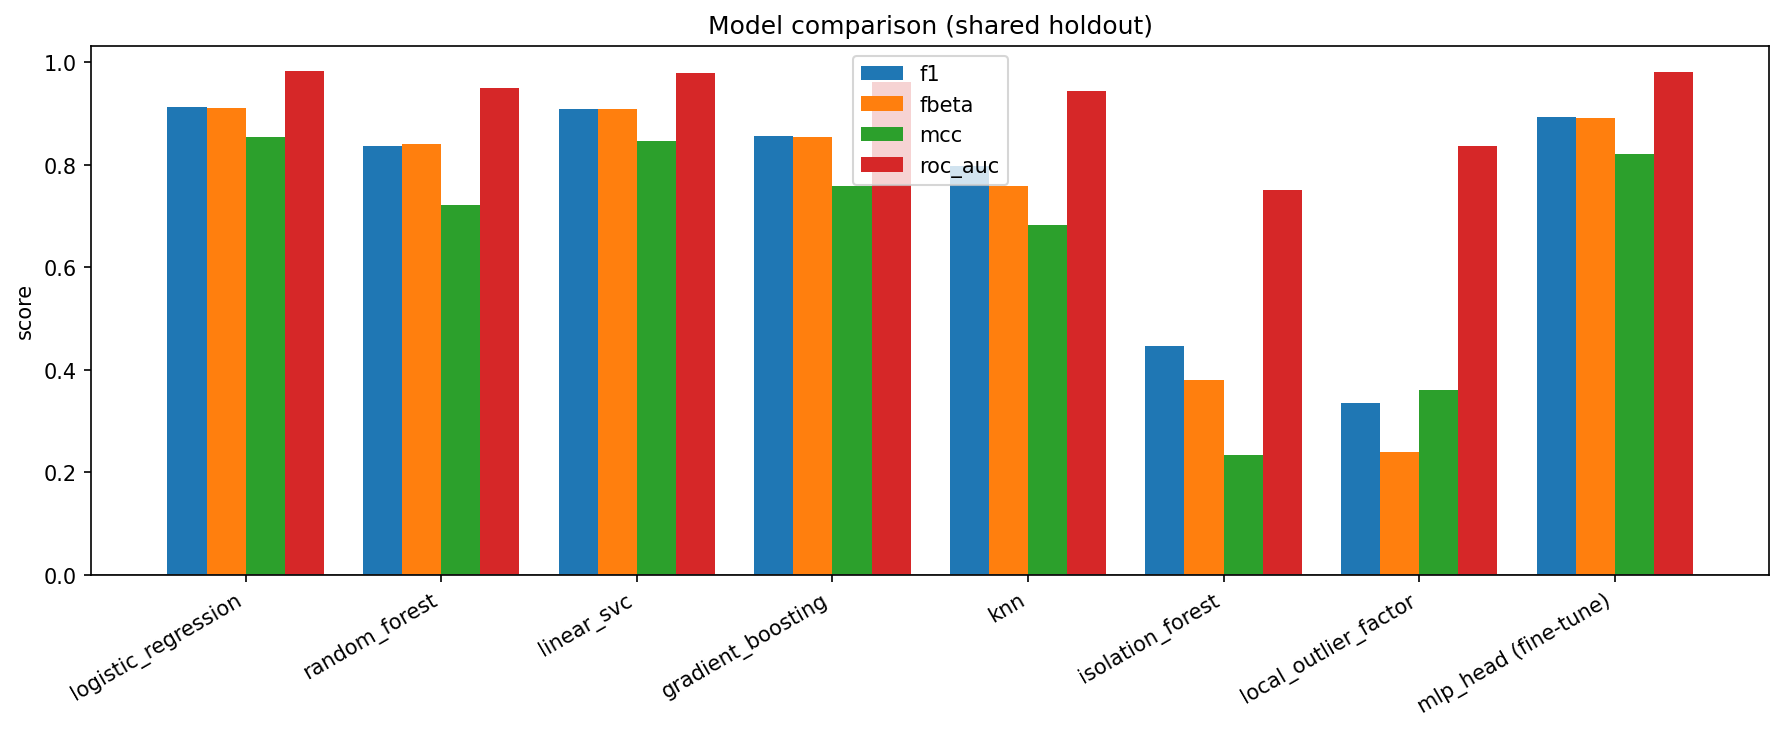
\includegraphics[width=\linewidth]{4_2_model_comparison_bars.png}
  \caption{F1, $\text{F}_2$, MCC and ROC--AUC per model on the shared holdout. The
  supervised linear models and the MLP head cluster at the top; the unsupervised
  detectors (right) collapse on the threshold metrics while retaining moderate ROC--AUC.}
  \label{fig:bars}
\end{figure}

\subsection{The embedding space}
Figure~\ref{fig:tsne} is the 2D t--SNE view referenced in Claim~3. There is genuine
structure---a large, near--pure normal cluster and many satellite clusters by request
type---but several satellites mix red and blue, so 2D separation is imperfect even though
the full--dimensional classifiers separate the classes well.

\begin{figure}[H]
  \centering
  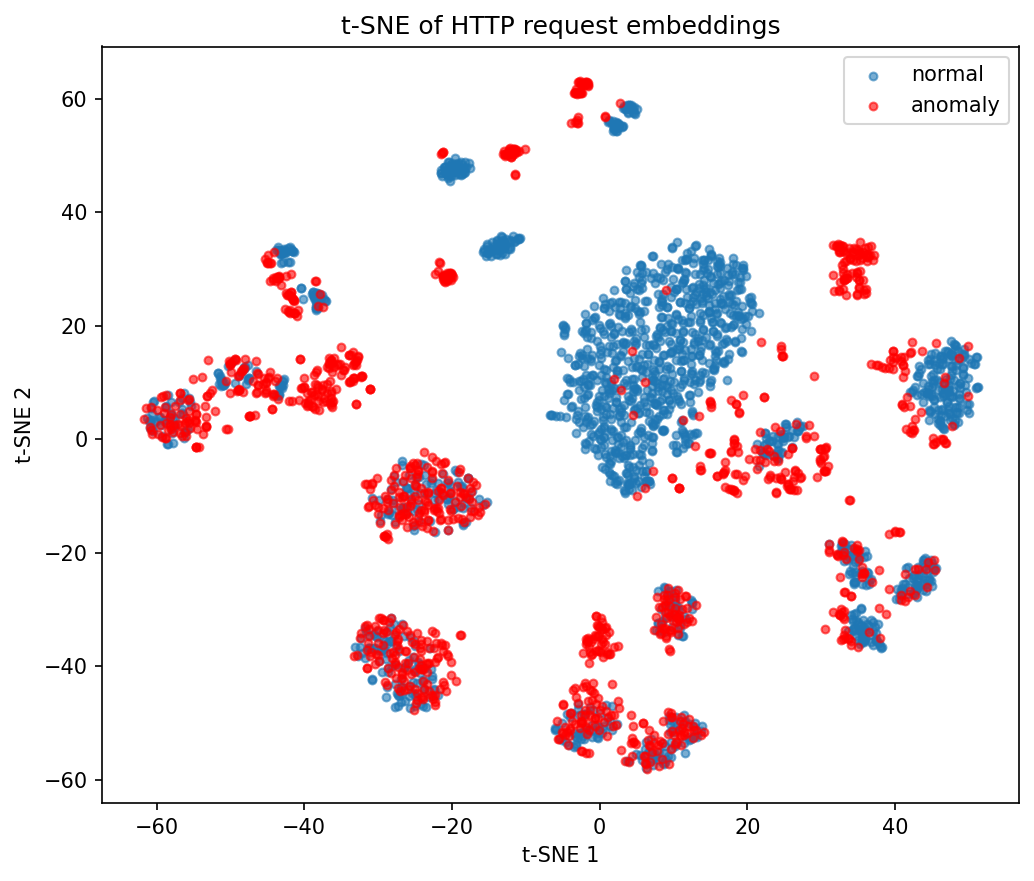
\includegraphics[width=0.72\linewidth]{3_2_tsne_embeddings.png}
  \caption{t--SNE of a $3{,}000$--request sample of the embeddings. Clear clustering by
  request type, one dominant normal cluster, but several clusters are class--mixed---so
  the ``well separated in 2D'' claim is only partially supported.}
  \label{fig:tsne}
\end{figure}

\subsection{Ranking quality and the best model}
The ROC overlay (Figure~\ref{fig:roc}) makes the ranking gap explicit: LR, linear SVC and
the MLP head sit on top (AUC $\approx0.98$), the tree/KNN models a step below, and the
unsupervised detectors far lower (Isolation Forest AUC $=0.75$). The best supervised
model's confusion matrix (Figure~\ref{fig:cm}) shows a well--balanced error profile---$247$
false positives vs $272$ false negatives---consistent with its high MCC.

\begin{figure}[H]
  \centering
  \begin{subfigure}{0.53\textwidth}
    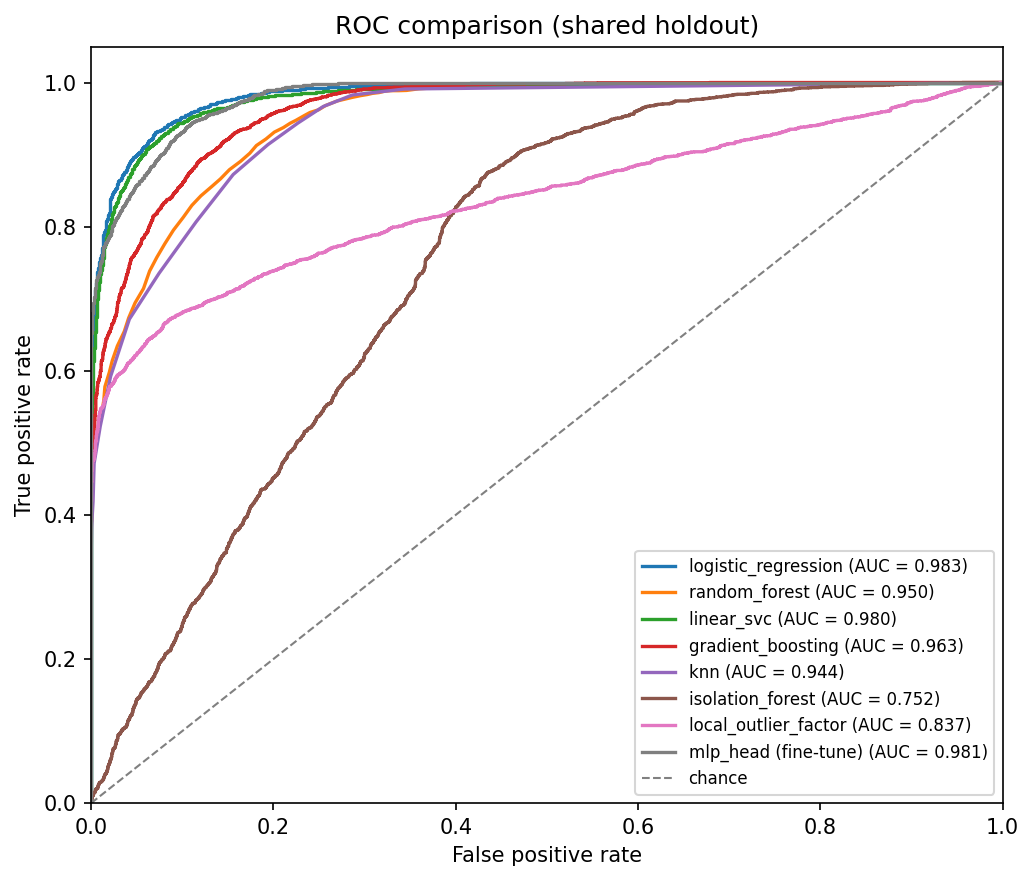
\includegraphics[width=\linewidth]{5_1_roc_comparison.png}
    \caption{ROC of all models (shared holdout).}
    \label{fig:roc}
  \end{subfigure}\hfill
  \begin{subfigure}{0.45\textwidth}
    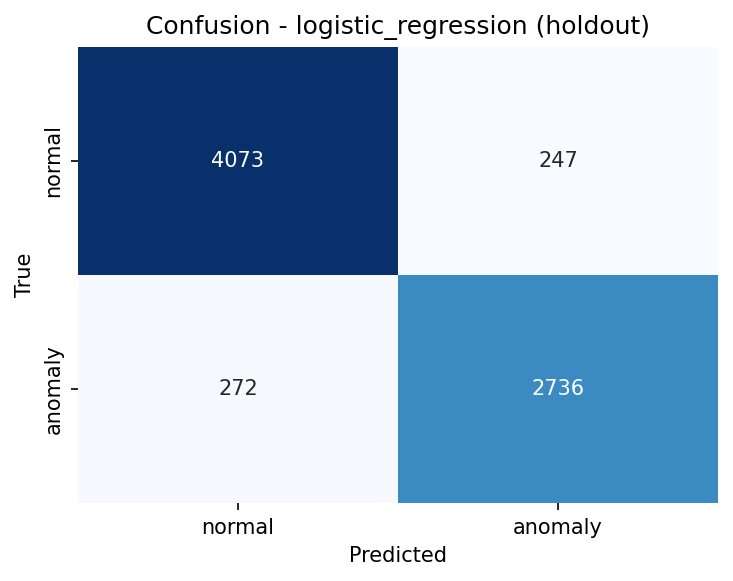
\includegraphics[width=\linewidth]{5_2_confusion_best_supervised.png}
    \caption{Confusion matrix, Logistic Regression.}
    \label{fig:cm}
  \end{subfigure}
  \caption{Threshold--free ranking (left) and the best supervised model's error profile
  (right).}
  \label{fig:roccm}
\end{figure}

\subsection{The trainable MLP head}
Figure~\ref{fig:mlp} shows the MLP head's learning curve: early stopping halted training
after 18 epochs at the best validation loss ($0.183$). The training loss keeps falling
while validation loss flattens with mild noise---the expected mild--overfitting signature
that early stopping is designed to catch. The head performs on par with the linear
models but does not exceed them, reinforcing that the representation, not the classifier,
is doing the heavy lifting.

\begin{figure}[H]
  \centering
  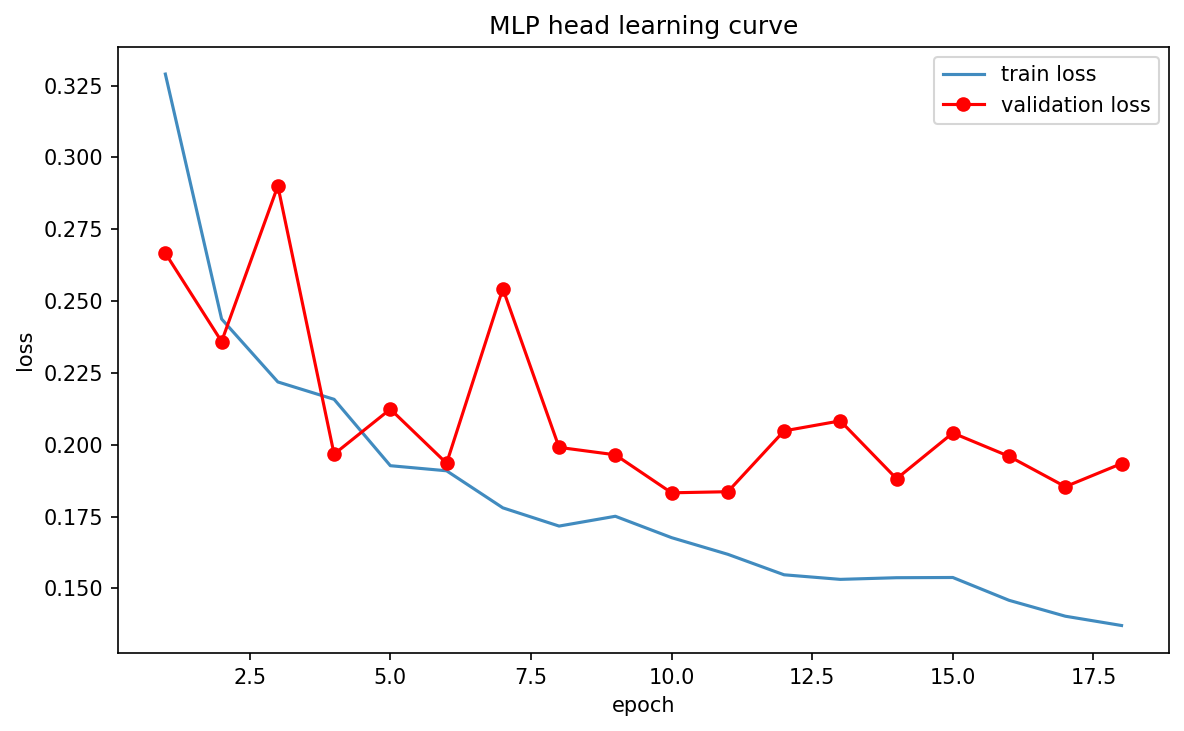
\includegraphics[width=0.72\linewidth]{4_1_mlp_learning_curve.png}
  \caption{MLP head learning curve (train vs validation loss). Early stopping restores the
  best--validation weights; the head matches but does not beat logistic regression.}
  \label{fig:mlp}
\end{figure}

\subsection{Reproduction vs the paper}
\label{sec:paper-vs-repro}
Table~\ref{tab:papervsrepro} compares our 5--fold CV numbers on CSIC~2010 with the paper's
(both use stratified 5--fold CV, so this is a fair comparison). The picture is consistent:
we \emph{reproduce the qualitative claim} (strong F1/MCC from simple classifiers on the
embeddings) but land a few F1 points lower and, on the operational tail metrics,
\emph{much} higher---our $\text{FPR}_{99}$ is $0.23$ vs the paper's $0.075$ for LR, and
$0.30$ vs $0.042$ for SVC. Our ranking also differs: the paper's best is SVC and its RF is
excellent ($\text{F1}=0.959$), whereas our best is LR and our RF is markedly weaker
($0.833$).

\begin{table}[H]
  \centering
  \footnotesize
  \setlength{\tabcolsep}{6pt}
  \begin{tabular}{lcccc}
    \toprule
    & \multicolumn{2}{c}{F1} & \multicolumn{2}{c}{$\text{FPR}_{99}$}\\
    \cmidrule(lr){2-3}\cmidrule(lr){4-5}
    Classifier & Paper & Repro & Paper & Repro\\
    \midrule
    Logistic Regression & 0.951 & 0.915 & 0.075 & 0.226\\
    Linear SVC          & 0.969 & 0.908 & 0.042 & 0.300\\
    Random Forest       & 0.959 & 0.833 & 0.070 & 0.322\\
    \bottomrule
  \end{tabular}
  \caption{Paper vs our reproduction on CSIC~2010 (stratified 5--fold CV). We reproduce the
  qualitative result but not the paper's low false--positive rates or its RF strength.}
  \label{tab:papervsrepro}
\end{table}

\noindent\textbf{Why the gap?} Several factors plausibly combine: (i) our reduced budget
(40\% data, 5 vs 10 epochs) yields a weaker language model and thus weaker embeddings;
(ii) our parser \emph{removes} the \texttt{\textbackslash r\textbackslash n} artifact the
paper exploited, making our test genuinely harder (and arguably more honest); (iii)
implementation differences (library versions, a histogram gradient--booster,
\texttt{max\_iter} settings); and (iv) tail metrics like $\text{FPR}_{99}$ are inherently
high--variance and degrade quickly when the embedding is even slightly weaker. The
direction of every one of these is ``our setup is harder/smaller'', which is exactly
consistent with reproducing the qualitative claim while under--shooting the exact numbers.

\section{Error Analysis}
\label{sec:error}

Because the unsupervised Isolation Forest scores the full inference set in order, we can
map its errors straight back to the original requests. Its confusion matrix on all
$24{,}426$ requests is $\text{TN}=12{,}344$, $\text{FP}=2{,}056$, $\text{FN}=6{,}584$,
$\text{TP}=3{,}442$: it misses roughly two--thirds of attacks (recall $0.34$). The score
distributions (Figure~\ref{fig:iforest}, left) explain why---the normal and anomaly score
densities overlap heavily, with only the normal mode cleanly resolved---so no threshold
separates them well. This is the visual counterpart of the low unsupervised numbers in
Table~\ref{tab:holdout}.

\begin{figure}[H]
  \centering
  \begin{subfigure}{0.55\textwidth}
    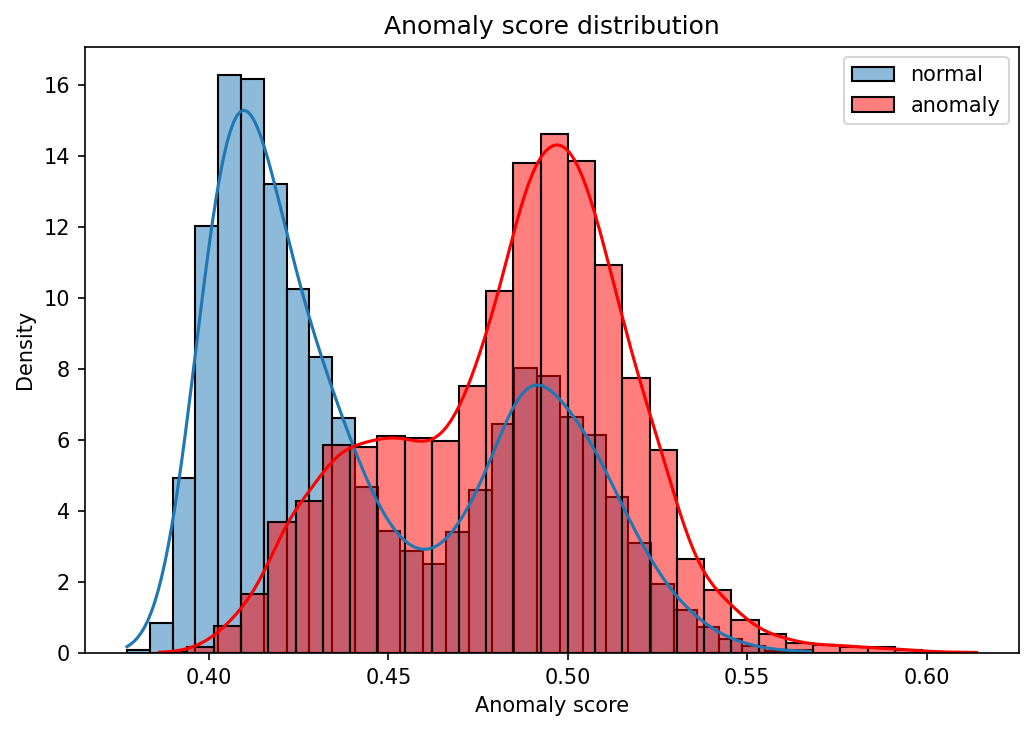
\includegraphics[width=\linewidth]{5_3_iforest_score_distribution.png}
    \caption{Anomaly--score densities by class.}
  \end{subfigure}\hfill
  \begin{subfigure}{0.43\textwidth}
    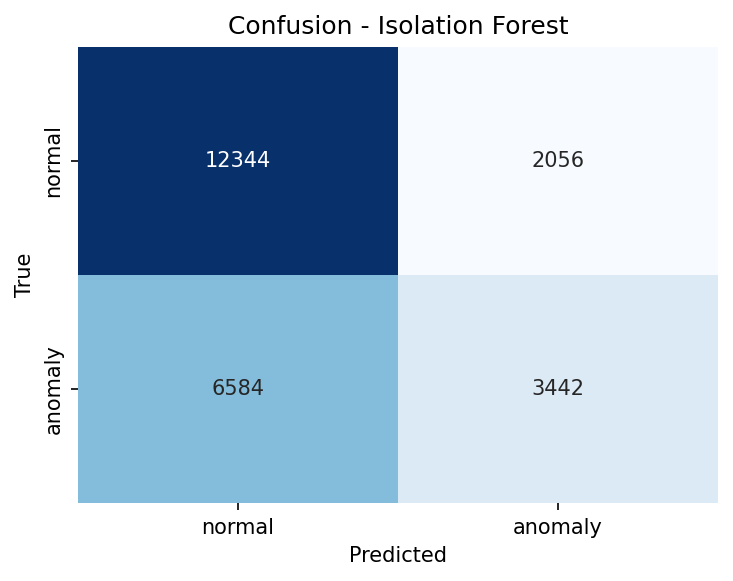
\includegraphics[width=\linewidth]{5_3_confusion_iforest.png}
    \caption{Confusion matrix (full inference set).}
  \end{subfigure}
  \caption{Isolation Forest error analysis. The heavy overlap of the score distributions
  (left) yields the poor confusion matrix (right): most attacks are missed.}
  \label{fig:iforest}
\end{figure}

\subsection{Examples of failures}
\paragraph{False positives (benign flagged as attack).} The flagged--benign requests are
legitimate, heavily parameterised e--commerce requests with percent--encoded accented
Spanish characters:
\begin{lstlisting}
GET /tienda1/publico/anadir.jsp?id=1&nombre=Jam%F3n+Ib%E9rico&precio=39&cantidad=41&B1=A%F1adir+al+carrito
POST /tienda1/publico/anadir.jsp
POST /tienda1/publico/caracteristicas.jsp
\end{lstlisting}
Their percent--encoding (\texttt{\%F3}, \texttt{\%E9}, \texttt{\%F1}) is benign but rare,
so a detector that learned ``normal traffic has little encoding'' treats them as
outliers.

\paragraph{False negatives (attacks missed).} The missed attacks structurally resemble
ordinary login / parameter traffic:
\begin{lstlisting}
GET /publico/autenticar.jsp?modo=entrar&login=bob%40%3CSCRipt%3Ealert%28Paros%29%3C%2FscrIPT%3E...&pwd=...
GET /publico/autenticar.jsp?modo=entrar&login=grimshaw&pwd=84m3ri156&rememberA=on&B1=Entrar
GET /publico/entrar.jsp?errorMsg=%2B
\end{lstlisting}
The first hides an XSS payload inside a \texttt{login} field; the others are near--normal
in shape. Because the request skeleton matches high--density normal regions, the
density--based detector places them among inliers.

\subsection{Patterns, implications and the FP/FN trade--off}
\textbf{Pattern.} The unsupervised detector errs on \emph{rare--but--benign encodings}
(false positives) and on \emph{low--footprint attacks that mimic normal structure} (false
negatives). The best \emph{supervised} model, by contrast, has a balanced and much smaller
error set ($247$ FP vs $272$ FN, Figure~\ref{fig:cm}), because labels teach it which rare
patterns are actually malicious. \textbf{Cybersecurity implication.} The false negatives
here include a real XSS attempt---exactly the failure that matters, since a missed XSS or
SQL injection is a potential breach; the false positives, while less dangerous, would (at
scale) erode operator trust and cause genuine alerts to be ignored. \textbf{Trade--off.}
The decision threshold on the continuous anomaly score is the single knob that trades
these off: lowering it raises recall (fewer missed attacks) at the cost of more false
alarms. This is precisely why we report $\text{FPR}_{90}$/$\text{FPR}_{99}$ and weight
recall with $\beta=2$---in an IDS we accept extra false alarms to avoid missing attacks,
but the reproduced $\text{FPR}_{99}\approx0.22$ shows that ``catch 99\% of attacks'' still
costs an operationally heavy false--alarm rate on this representation.

\section{Conclusions}
\label{sec:conclusions}

\subsection{Claim verdicts at a glance}
Table~\ref{tab:claims} summarises the critical evaluation of Section~\ref{sec:critical}
against our evidence.

\begin{table}[H]
  \centering
  \footnotesize
  \renewcommand{\arraystretch}{1.25}
  \begin{tabular}{p{5.4cm} p{2.7cm} p{6.6cm}}
    \toprule
    \textbf{Author's claim} & \textbf{Verdict} & \textbf{Evidence from our reproduction}\\
    \midrule
    RoBERTa embeddings give SOTA \emph{supervised} detection &
    Partially supported &
    Reproduced $\text{F1}=0.91$, $\text{ROC--AUC}=0.98$; but $\text{FPR}_{99}$ far higher
    than the paper, and ``SOTA'' is weakened by leakage.\\
    Representation is unsupervised / suits label--free use &
    Not supported &
    Isolation Forest $\text{F1}=0.45$, LOF $\text{F1}=0.34$ on the same embeddings.\\
    Classes ``well separated'' in 2D (t--SNE) &
    Partially supported &
    Clear clustering, but many satellite clusters are class--mixed (Fig.~\ref{fig:tsne}).\\
    Near--perfect scores on CSE--CIC--IDS2018 &
    Artifact, not method quality &
    The authors' own analysis attributes it to fixed \texttt{Accept} headers (leakage).\\
    Method is interpretable &
    Plausible (not tested) &
    Out of scope here; the token--removal technique is sound but costly.\\
    Evaluation methodology is appropriate &
    Mostly, with caveats &
    Good CV/metrics/leakage control; but unrealistic 41\% base rate and dataset
    artifacts inflate results.\\
    \bottomrule
  \end{tabular}
  \caption{Verdicts on the paper's main claims.}
  \label{tab:claims}
\end{table}

\subsection{Key findings}
\begin{itemize}[nosep,leftmargin=1.4em]
  \item The paper's core idea works: a RoBERTa MLM trained on normal HTTP traffic produces
        embeddings on which \emph{simple, linear} supervised classifiers achieve strong
        detection ($\text{F1}=0.91$, $\text{MCC}=0.85$, $\text{ROC--AUC}=0.98$), even at
        40\% data and 5 epochs.
  \item Unsupervised detection on those same embeddings is weak (F1 $=0.34$--$0.45$),
        contradicting the paper's optimistic outlook.
  \item The embedding is highly redundant---$\sim$14 PCA components capture 90\% of
        variance---so the paper's ``too large'' limitation is real and fixable.
  \item Much of CSIC~2010's apparent easiness comes from artifacts (CRLF terminators,
        \texttt{PUT}--only--in--anomalies, 64\% duplicate fingerprints) and an unrealistic
        41\% attack prevalence.
\end{itemize}

\subsection{Lessons learned}
The representation, not the classifier, is what matters: a good embedding makes logistic
regression competitive with an MLP, while a bad task setup (unrealistic base rate, leaked
artifacts) can make \emph{any} classifier look near--perfect. Critically evaluating a
security paper therefore means interrogating the \emph{data and metrics} at least as hard
as the model---the most impressive numbers in this literature are often the least
trustworthy.

\subsection{Strengths and weaknesses of the proposed solution}
\textbf{Strengths:} no hand--crafted features or OOV problem; trains on normal traffic
only; strong, near--linear separability; genuine interpretability mechanism; honest
reporting of artifacts. \textbf{Weaknesses:} very large ($\sim$3000--d) and redundant
representation; heavy compute (hours on multiple GPUs); detection is really supervised
despite the ``unsupervised representation'' framing; results validated only on
artifact--laden benchmarks at unrealistic base rates; no temporal / drift evaluation.

\subsection{Suggestions for future improvements}
Compress the embedding with PCA/agglomeration ($3072\!\rightarrow\!\sim\!50$) to cut cost
with negligible accuracy loss; evaluate at realistic ($\ll1\%$) attack base rates and
report precision/PR--AUC there; add response--side and session/rate features; test true
generalisation on modern, non--artifactual traffic and across time; and, if unsupervised
detection is the goal, pursue density models in the \emph{reduced} space or one--class
objectives rather than assuming the supervised embedding transfers.

\section{Executive Summary}
\label{sec:exec}

\textbf{Problem and source.} We reproduced and critically evaluated \emph{HTTP2vec}
(Gniewkowski et al., 2021), which tackles web--attack detection by treating each HTTP
request as text. A byte--level BPE tokenizer and a RoBERTa masked--language model are
trained on \emph{normal} traffic; every request is embedded as the mean of its last four
hidden layers ($3072$--d); and simple classifiers (Logistic Regression, Random Forest,
linear SVC) label the embeddings as normal or anomalous. The paper reports up to
$\text{F1}=0.969$ on CSIC~2010 and a ``perfect'' $\text{F1}=0.999$ on CSE--CIC--IDS2018,
and highlights interpretability and clustering as key benefits.

\textbf{What we did.} We built an independent, modular re--implementation of the whole
pipeline and ran it end--to--end on CSIC~2010 (a seeded 40\% subset, 5 epochs, single GPU).
Beyond reproducing the paper's three classifiers, we added gradient boosting, KNN, a
second unsupervised detector (LOF alongside Isolation Forest) and a trainable MLP head, and
we scored \emph{all} models on one shared, seeded, stratified holdout. We performed full
EDA (class balance, distributions, Spearman correlation, duplicate and crosstab analysis),
a feature--engineering analysis (encoding, pooling, scaling, PCA), and an error analysis.

\textbf{Headline results.} The paper's central idea holds: on the embeddings, Logistic
Regression is best with $\text{F1}=0.913$, $\text{MCC}=0.853$ and $\text{ROC--AUC}=0.983$,
with linear SVC and our MLP head close behind---confirming the space is nearly linearly
separable. However, we did not reproduce the paper's low false--positive rates
($\text{FPR}_{99}\approx0.22$ for us vs $0.075$ reported), and the two \emph{unsupervised}
detectors were weak ($\text{F1}=0.45$ and $0.34$), directly contradicting the paper's
speculation that unsupervised detection on these embeddings ``is likely to be effective''.
PCA showed the $3072$--d representation is highly redundant ($\sim$14 components reach 90\%
variance).

\textbf{Critical assessment.} Several of the paper's most striking results are driven by
the \emph{data}, not the method: the ``perfect'' IDS2018 score is a header--leakage
artifact (the authors themselves show this); CSIC~2010 contains CRLF--terminator and
HTTP--method giveaways and 64\% duplicate request fingerprints; and the 41\% attack
prevalence is far above any real deployment, inflating precision, F1 and accuracy. The
evaluation protocol is otherwise sound (stratified CV, appropriate metrics, no
train/inference leakage on the normal side, which we verified in code).

\textbf{Bottom line.} HTTP2vec is a genuinely good \emph{supervised} feature extractor for
HTTP anomaly detection and we recommend it for that use---given labels, a GPU, dimensionality
reduction and, above all, careful guarding against dataset artifacts and base--rate
mismatch. Its unsupervised promise, its exact SOTA numbers, and its ``clean 2D
separation'' narrative are not supported by our reproduction.

\section{Summing It Up}
\label{sec:summing}

\begin{description}[leftmargin=0pt,style=nextline]
  \item[Problem addressed] Detecting anomalous / attack HTTP requests (SQL injection, XSS,
        CRLF, etc.)---a Web Application Firewall / IDS problem.
  \item[Selected source] \emph{HTTP2vec: Embedding of HTTP Requests for Detection of
        Anomalous Traffic}, Gniewkowski, Maciejewski, Surmacz, Walentynowicz, arXiv:2108.01763 (2021).
  \item[Dataset] CSIC~2010 HTTP dataset (normal training / normal inference / anomalous
        inference); our run used a seeded 40\% subset ($14{,}400$ / $14{,}400$ / $10{,}026$).
  \item[Methodology] BBPE tokenizer $+$ RoBERTa MLM on normal traffic $\rightarrow$
        $3072$--d embeddings $\rightarrow$ supervised classifiers and unsupervised
        detectors; independent re--implementation, evaluated with stratified CV and a shared
        holdout using F1, $\text{F}_2$, MCC, ROC--AUC and FPR@TPR.
  \item[Main findings] Strong supervised detection reproduced ($\text{F1}=0.91$,
        $\text{AUC}=0.98$); weak unsupervised detection ($\text{F1}=0.34$--$0.45$); highly
        redundant embedding; substantial dataset artifacts and an unrealistic base rate.
  \item[Were the claims supported?] Partially. The supervised--detection claim: yes,
        qualitatively. The exact SOTA numbers, the unsupervised outlook, and the clean 2D
        separation: no. The IDS2018 ``perfect'' result: an artifact.
  \item[Most important insight] In security ML the data and the metrics deserve more
        scrutiny than the model; impressive benchmark numbers here largely reflect
        leakage and prevalence, not real--world detection power.
  \item[Do we recommend this approach for similar problems?] Yes, as a \emph{supervised}
        HTTP representation, with the caveats above (labels, GPU, dimensionality reduction,
        artifact/base--rate control). No, as an off--the--shelf \emph{unsupervised} detector.
  \item[Final conclusion] HTTP2vec is a sound and useful idea whose core supervised claim
        we independently reproduce, but whose headline results are optimistic; a rigorous,
        artifact-- and base--rate--aware evaluation is essential before trusting such numbers
        in production.
\end{description}

\end{document}
